\documentclass[11pt]{article}
%基于北京航空航天大学仪器科学与光电工程学院实验报告及课程报告排版得来,类似于毕业论文排版格式
%后续将更新毕业论文排版格式
\usepackage{graphicx,float}%使用图的宏包,使用图的浮动体宏包,引入参数H使图像紧跟当前文字
\usepackage{caption} %使用图表标题的宏包
\usepackage[colorlinks=true,pdfstartview=FitH,%
linkcolor=black,anchorcolor=violet,citecolor=magenta]{hyperref}%加载hyperref宏包,使用超链接
\usepackage{setspace}%用于设置行间距列间距等命令的宏包
\usepackage{array}%设置列表高度宽度的宏包
\usepackage{zhnumber}%使用中文数字编号的宏包
\usepackage{titlesec,titletoc}%使用标题自定义形式的宏包和使用目录自定义形式的宏包
\usepackage{siunitx}%物理学单位宏包
\usepackage{tabularx}%让表格宽度等于页面宽度
\usepackage{makecell}%单个表格单元调整的宏包
\usepackage{subfigure} %%使用子图的宏包
\usepackage[backend=biber,bibstyle=gb7714-1987,%nature,%%加载biblatex宏包,使用参考文献
citestyle=gb7714-1987%,backref=true%%其中后端backend使用biber
,url=false
]{biblatex}%标注(引用)样式citestyle,著录样式bibstyle都采用gb7714-2015样式
% \usepackage{pgfplots}%类似tikz的一个画图库,主要画统计图
\usepackage{../customStyle}
% \usepackage{customFont}%自行编写的字体命令库,基于CJK宏包
% \usepackage{bh_style}%自行编写的风格文件,基于使用习惯和格式要求
% \usepackage{math_formulate}%自行编写的数学公式命令库,基于amsmath宏包
% \usepackage{picture}%集成图形绘制库,主要包括了tikz和pgfplots两大主流宏包
% \usepackage[lite,subscriptcorrection,slantedGreek,nofontinfo]{mtpro2}%使用mathtimepro2商业字体作为数学环境,并不推荐

%biblatex宏包的参考文献数据源加载方式,注意book.bib应当与.tex文件在同一目录下,不然有可能会报错
\addbibresource[location=local]{book.bib}
% % \bibliographystyle{gbt7714-numerical}
%%% 下面的命令重定义页面边距,使其符合中文刊物习惯 %%%%
% \addtolength{\topmargin}{2.5cm}
\setlength{\oddsidemargin}{0.63cm}  % 3.17cm - 1 inch
\setlength{\evensidemargin}{\oddsidemargin}
% \setlength{\textwidth}{14.66cm}
% \setlength{\textheight}{24.00cm}    % 24.62

\graphicspath{{./fig}}

\begin{document}
\pagenumbering{Roman}

\setcounter{tocdepth}{3}
%设定目录深度                      
\tableofcontents
%列出目录
\newpage
\pagenumbering{arabic}
\section{多视图几何知识点}
\subsection{齐次坐标二维点、二维线的表示,齐次坐标二维点和线的关系(相交、点在线上、交点交线)P20}
设齐次点为$\mathbold{x}=(x_1,x_2,x_3)^T$,齐次线为$\mathbold{l}=(l_1,l_2,l_3)^T$,其中点和线都是二维的,则从齐次点退化为非齐次点可用下式:
\begin{equation*}
  \mathbold{x}=(x_1,x_2,x_3)^T=\circbrac{\frac{x_1}{x_3},\frac{x_2}{x_3}}^T
\end{equation*}\par
点在直线上:
\begin{equation*}
  \mathbold{x}^T\mathbold{l}=0
\end{equation*}\par
两个齐次点确定一条直线:
\begin{equation*}
  \mathbold{l}=\mathbold{x}\times\mathbold{x}'
\end{equation*}\par
两条齐次线确定一个点:
\begin{equation*}
  \mathbold{x}=\mathbold{l}\times\mathbold{l}'
\end{equation*}\par
\subsection{什么是理想点?P21}
理想点就是位于无穷远直线或者无穷远平面上的点,又称消隐点,其齐次坐标的最后一个坐标值为0。
\subsection{二维二次曲线的表示、对偶二次曲线与二次曲线的关系,二次曲线切线切点怎么表示?P23}
二维二次曲线的表示:
\begin{equation*}
  \mathbold{C}=\begin{bmatrix}
    a   & b/2 & d/2 \\
    b/2 & c   & e/2 \\
    d/2 & e/2 & f
  \end{bmatrix}
\end{equation*}\par
点在二次曲线上的表示:
\begin{equation*}
  \mathbold{x}^T\mathbold{C}\mathbold{x}=0
\end{equation*}\par
对偶二次曲线:二次曲线上的全部切线所形成的包络,即符合以下公式:
\begin{equation*}
  \mathbold{l}^T\mathbold{C}^*\mathbold{l}=0
\end{equation*}\par
对偶二次曲线等于二次曲线的伴随矩阵,当二次曲线可逆时,该伴随矩阵在齐次意义下等于二次曲线的逆矩阵。\par
经过二次曲线上某一点的切线可表示为:
\begin{equation*}
  \mathbold{l=Cx}
\end{equation*}
\subsection{退化二次曲线P24}
退化二次曲线是不满秩的二次曲线,当秩为2时,可以表示为两条直线的乘积,即:
\begin{equation*}
  \mathbold{C}=\mathbold{ml}^T+\mathbold{lm}^T
\end{equation*}\par
当秩为1时,二次曲线退化为一个重合的点。
\subsection{二次曲线极点-极线关系、共轭概念、仿射分类P44}
二次曲线外一点$\mathbold{x}$可作二次曲线两条切线$\mathbold{l}_1,\mathbold{l}_2$,两切点$\mathbold{x}_1,\mathbold{x}_2$确定一条直线$\mathbold{l}=\mathbold{l_1}\times\mathbold{l}_2$,该直线称为极线,点$\mathbold{x}$称为极点,二者具有以下的关系:
\begin{equation*}
  \mathbold{l}=\mathbold{Cx}
\end{equation*}\par
因此又有以下的关系,称为共轭关系:
\begin{equation*}
  \mathbold{l}^T\mathbold{C}\mathbold{x}=0
\end{equation*}\par
二次曲线根据其仿射性质可以分为三类,如下表:
\begin{table}[H]
  \centering
  \caption{二次曲线的仿射分类}
  \begin{tabular}{|c|c|c|c|}
    \hline
    二次曲线     & 圆(椭圆) & 抛物线 & 双曲线 \\
    \hline
    与无穷远直线交点 & 0个    & 1个  & 2个  \\
    \hline
  \end{tabular}
\end{table}
\subsection{点变换、直线协变、二次曲线协变、对偶二次曲线逆变P27}
在单应$\mathbold{H}$作用下,点$\mathbold{x}$变换为$\mathbold{x}'$,则有:
\begin{equation*}
  \mathbold{x}'=\mathbold{Hx}
\end{equation*}\par
直线$\mathbold{l}$变换为$\mathbold{l}'$,则有:
\begin{equation*}
  \mathbold{l}'=\mathbold{H}^{-T}\mathbold{l}
\end{equation*}\par
二次曲线$\mathbold{C}$变换为$\mathbold{C}'$,则有:
\begin{equation*}
  \mathbold{C}'=\mathbold{H}^{-T}\mathbold{CH}^{-1}
\end{equation*}\par
对偶二次曲线$\mathbold{C}^*$变换为$\mathbold{C}^{*'}$,则有:
\begin{equation*}
  \mathbold{C}^{*'}=\mathbold{HC}^*\mathbold{H}^T
\end{equation*}\par
由于直线和二次曲线的变换中含有$\mathbold{H}^{-1}$项,因此又称为协变。
\subsection{四类变换的性质及其变换矩阵P30}
欧氏变换,又称刚体变换,不改变原始形状的长度和夹角,其变换矩阵为:
\begin{equation*}
  \mathbold{H}=\begin{bmatrix}
    \mathbold{R}   & \mathbold{t} \\
    \mathbold{0}^T & 1
  \end{bmatrix}
\end{equation*}\par
其中,$\mathbold{R}$为旋转矩阵,$\mathbold{t}$为平移向量。\par
相似变换,又称等距变换,不改变原始形状的夹角,其变换矩阵为:
\begin{equation*}
  \mathbold{H}=\begin{bmatrix}
    s\mathbold{R}  & \mathbold{t} \\
    \mathbold{0}^T & 1
  \end{bmatrix}
\end{equation*}\par
其中增加了一项缩放因子$s$,是对整个图像的均匀缩放。\par
仿射变换,不改变原始形状的平行性,变换矩阵为:
\begin{equation*}
  \mathbold{H}=\begin{bmatrix}
    \mathbold{A}   & \mathbold{t} \\
    \mathbold{0}^T & 1
  \end{bmatrix}
\end{equation*}\par
其中矩阵$\mathbold{A}$是一个非奇异的矩阵。\par
射影变换,不改变原始形状的直线性,变换矩阵为:
\begin{equation*}
  \mathbold{H}=\begin{bmatrix}
    \mathbold{A}   & \mathbold{t} \\
    \mathbold{v}^T & 1
  \end{bmatrix}
\end{equation*}\par
其中矩阵$\mathbold{A}$是一个非奇异的矩阵,向量$\mathbold{v}$是非零向量。
\subsection{	射影变换阵的分解P32}
射影矩阵可以分解为三个独立的变换,即:
\begin{equation*}
  \mathbold{H}=\begin{bmatrix}
    s\mathbold{R}  & \mathbold{t} \\
    \mathbold{0}^T & 1
  \end{bmatrix}
  \begin{bmatrix}
    \mathbold{K}   & \mathbold{0} \\
    \mathbold{0}^T & 1
  \end{bmatrix}
  \begin{bmatrix}
    \mathbold{I}   & \mathbold{0} \\
    \mathbold{v}^T & 1
  \end{bmatrix}
  \triangleq\mathbold{H}_S\mathbold{H}_A\mathbold{H}_P
\end{equation*}\par
其中,$\mathbold{H}_P$仅改变图像的无穷远直线(射影变换),$\mathbold{H}_A$是仅改变比例尺的长宽比(仿射变换),$\mathbold{H}_S$是相似变换。\par
射影变换的逆变换矩阵也是一个射影变换,因此也可以分解成类似的结果,通常将它们反着写,即:
\begin{equation*}
  \mathbold{H}'=\mathbold{H}'_P\mathbold{H}'_A\mathbold{H}'_S
\end{equation*}\par
\subsection{	两种恢复至仿射变换的方法P37}
恢复至仿射变换,需要将无穷远直线校正至规范位置,因此需要求出图像的无穷远直线即可:
\begin{itemize}
  \item 通过两对平行线的交点求出无穷远直线;
  \item 通过交比不变,作图求出无穷远直线。
\end{itemize}
\subsection{三种恢复至相似变换的方法P41}
恢复至仿射变换,需要将绝对对偶二次曲线校正至规范位置,因此需要求出绝对对偶二次曲线:
\begin{itemize}
  \item 通过五正交直线;
  \item 在仿射校正的基础上,通过两对正交直线即可校正;
  \item 在仿射校正的基础上,通过一个椭圆或者一个已知长度的交比来计算校正。
\end{itemize}
\subsection{三维点和平面的齐次式以及关联定义、对偶定义,平面点的参数方程表示P50}
三维点定义:$\mathbold{X}=(X_1,X_2,X_3,X_4)^T$,平面定义为:$\mathbold{\pi}=(\pi_1,\pi_2,\pi_3,\pi_4)^T$,点在平面上,可有以下关系:
\begin{equation*}
  \mathbold{\pi}^T\mathbold{X}=0
\end{equation*}\par
平面点的参数方程表示:
\begin{equation*}
  \mathbold{X}=\mathbold{Mx}
\end{equation*}\par
式中,$\mathbold{M}$是平面$\mathbold{\pi}$的零空间,是一个$4\times3$的矩阵,$\mathbold{x}$是一个三维齐次向量,即参数。
\subsection{	空间直线的生成子空间表示和零空间表示、平面与直线的交点以及包含一条直线和点的平面定义方法P52}
两个空间点构成矩阵:
\begin{equation*}
  \begin{bmatrix}
    \mathbold{X}_1^T \\
    \mathbold{X}_2^T
  \end{bmatrix}
\end{equation*}\par
空间直线是它的生成子空间,即:
\begin{equation*}
  \mathbold{X}=\lambda_1\mathbold{X}_1+\lambda_2\mathbold{X}_2
\end{equation*}\par
空间直线也可以使用两个平面的零空间表示,即:
\begin{equation*}
  \begin{bmatrix}
    \mathbold{\pi}_1^T \\
    \mathbold{\pi}_2^T
  \end{bmatrix} \mathbold{l}=0
\end{equation*}\par
平面与直线的交点,相当于三个平面交于一点,需要使用零空间表示,即:
\begin{equation*}
  \begin{bmatrix}
    \mathbold{\pi}_1^T \\
    \mathbold{\pi}_2^T \\
    \mathbold{\pi}_3^T
  \end{bmatrix} \mathbold{X}=0
\end{equation*}\par
直线与一点共面,相当于三个点位于平面上,需要使用生成子空间表示 ,即:
\begin{equation*}
  \begin{bmatrix}
    \mathbold{X}_1^T \\
    \mathbold{X}_2^T \\
    \mathbold{X}_3^T
  \end{bmatrix} \mathbold{\pi}=0
\end{equation*}\par
\subsection{使用Plücker矩阵定义的直线以及对偶直线,直线和平面的关联P53}
直线的Plücker矩阵定义(下文中全部大写的L均表示Plücker形式的直线):
\begin{equation*}
  \mathbold{L}=\mathbold{X}_1\mathbold{X}_2^T-\mathbold{X}_2\mathbold{X}_1^T
\end{equation*}\par
对偶直线的Plücker矩阵定义:
\begin{equation*}
  \mathbold{L}^*=\mathbold{\pi}_1\mathbold{\pi}_2^T-\mathbold{\pi}_2\mathbold{\pi}_1^T
\end{equation*}\par
直线与平面交于一点,即:
\begin{equation*}
  \mathbold{X}=\mathbold{L}^T\mathbold{\pi}
\end{equation*}\par
直线和一点共面,即:
\begin{equation*}
  \mathbold{\pi}=\mathbold{L}^T\mathbold{X}
\end{equation*}\par
\subsection{两直线相交的充要条件以及三个推论P54}
两直线相交的充要条件是两直线的双线性乘积为零,即:
\begin{equation*}
  \mathcal{L_1\sep L_2}=\det\circbrac{\mathbold{X}_1,\mathbold{X}_2,\mathbold{X}_3,\mathbold{X}_4}=0
\end{equation*}\par
三个推论分别是:
\begin{itemize}
  \item 一条直线和另一条直线的对偶形式已知,则可以写出:\\
        $\circbrac{\mathbold{\pi}_1^T\mathbold{X}_1}\cdot\circbrac{\mathbold{\pi}_2^T\mathbold{X}_2}-\circbrac{\mathbold{\pi}_2^T\mathbold{X}_1}\cdot\circbrac{\mathbold{\pi}_1^T\mathbold{X}_2}=0$
  \item 使用两平面表示的直线也可以得到相同的双线性乘积结果:\\
        $\mathcal{L_1\sep L_2}=\det\circbrac{\mathbold{\pi}_1,\mathbold{\pi}_2,\mathbold{\pi}_3,\mathbold{\pi}_4}=0
        $
  \item 六维向量$\mathcal{L}=[l_{12},l_{12},l_[14],l_{23},l_{24},l_{34}]^T$仅表示一条三维直线,当且仅当双线性乘积为零。
\end{itemize}
\subsection{	绝对二次曲线、度量两空间直线的夹角,四个关于绝对二次曲线的性质P61}
绝对二次曲线定义为符合以下公式的全部点的集合:
\begin{align*}
  \left\{
  \begin{aligned}
    x_1^2+x_2^2+x_3^2 & =0 \\
    x_4               & =0
  \end{aligned}
  \right.
\end{align*}\par
在规范位置处,绝对二次曲线可以表示为:
\begin{equation*}
  \mathbold{\Omega}_\infty=\begin{bmatrix}
    1 & 0 & 0 & 0 \\
    0 & 1 & 0 & 0 \\
    0 & 0 & 1 & 0 \\
    0 & 0 & 0 & 0
  \end{bmatrix}
\end{equation*}\par
求解两空间直线的夹角,可以使用以下公式:
\begin{equation*}
  \cos\theta=\frac{\mathbold{L}_1^T\mathbold{\Omega}_\infty\mathbold{L}_2}{\sqrt{\mathbold{L}_1^T\mathbold{\Omega}_\infty\mathbold{L}_1}\sqrt{\mathbold{L}_2^T\mathbold{\Omega}_\infty\mathbold{L}_2}}
\end{equation*}\par
四点关于绝对二次曲线的性质:
\begin{itemize}
  \item 绝对二次曲线与直线交于两个虚球点;
  \item 绝对二次曲线与任意的圆交于两个虚球点;
  \item 绝对二次曲线与任意的球交于无穷远平面;
  \item 绝对二次曲线在相似变换作用下保持集合不变,而不是点点不变。
\end{itemize}
\subsection{绝对对偶二次曲面、度量两平面夹角P63}
绝对对偶二次曲面是绝对二次曲线全部切平面的包络,表示为:
\begin{equation*}
  \mathbold{Q}^*_\infty=\begin{bmatrix}
    1 & 0 & 0 & 0 \\
    0 & 1 & 0 & 0 \\
    0 & 0 & 1 & 0 \\
    0 & 0 & 0 & 0
  \end{bmatrix}
\end{equation*}\par
度量两平面的夹角,可以使用以下公式:
\begin{equation*}
  \cos\theta=\frac{\mathbold{\pi}_1^T\mathbold{Q}^*_\infty\mathbold{\pi}_2}{\sqrt{\mathbold{\pi}_1^T\mathbold{Q}^*_\infty\mathbold{\pi}_1}\sqrt{\mathbold{\pi}_2^T\mathbold{Q}^*_\infty\mathbold{\pi}_2}}
\end{equation*}\par
绝对对偶二次曲面在相似变换下保持不变。
\subsection{摄像机的中心、图像平面、主轴、主点、主平面P117}
投影中心称为摄像机的中心,记为$\mathbold{C}$;\par
摄像机的主轴定义为,过摄像机中心且与摄像机光轴平行的矢量方向;\par
图像平面定义为,与摄像机中心保持焦距位置处,与主轴垂直的平面;\par
摄像机的主点定义为,摄像机主轴与图像平面的交点;\par
摄像机的主平面定义为,经过摄像机\textbf{中心}且与摄像机主轴垂直的平面。\par
\subsection{摄像机投影矩阵P的四种写法、内参数和外参数P118}
摄像机投影矩阵可以写为以下四种形式:
\begin{itemize}
  \item 标准形式(世界坐标系与相机坐标系重合):$\mathbold{P}=\mathbold{K[I\sep 0]}$;
  \item 当世界坐标系与相机坐标系不重合时,使用相机的中心表示为:$\mathbold{P}=\mathbold{K[R\sep -R\tilde{C}]}$;
  \item 将内参数矩阵和外参数矩阵分离的形式,写为:$\mathbold{P}=\mathbold{KR}\mathbold{[I\sep -\tilde{C}]}$;
  \item 保留最后一列的形式:$\mathbold{P}=\mathbold{M}\mathbold{[I\sep M^{-1}p_4]}$。
\end{itemize}\par
第二种形式给出了内参数和外参数的定义,内参数矩阵为:$\mathbold{K}$;外参数矩阵为$\mathbold{[R\sep t]}$。
\subsection{解读标定矩阵P,摄像机中心、列向量含义、行向量含义、主平面、轴平面、主点以及主射线的数学表示P121}
记标定矩阵$\mathbold{P}$为:
\begin{equation*}
  \mathbold{P}=\begin{bmatrix}
    P_1^T \\\\
    P_2^T \\\\
    P_3^T
  \end{bmatrix}
  =\begin{bmatrix}
    p_1 & p_2 & p_3 & p_4
  \end{bmatrix}=\begin{bmatrix}
    p_{11} & p_{12} & p_{13} & p_{14} \\
    p_{21} & p_{22} & p_{23} & p_{24} \\
    p_{31} & p_{32} & p_{33} & p_{34}
  \end{bmatrix}
\end{equation*}\par
投影矩阵的行向量$P_1^T,P_2^T$代表图像上x轴和y轴的与相机主轴形成的两个平面,称为轴平面;第三行$P_3^T$代表相机的主平面;\par
投影矩阵的列向量$p_1,p_2,p_3$代表相机对世界坐标系x轴、y轴、z轴成像所得到的像点;第四列向量$p_4$代表相机对世界坐标系坐标原点的图像;\par
相机的中心是两个轴平面与主平面的交点,因此可以使用标定矩阵$\mathbold{P}$的零空间来表示:$\mathbold{C}=\mathcal{N}(\mathbold{P})$;\par
摄像机的主点是主轴向量对主平面的交点,主轴向量是主平面的法向量,因此是投影矩阵第三行的无穷远点,即$[p_{31},p_{32},p_{33},0]^T$,相机对该无穷远点成像即为主点,书上取前三项为$m_3$,因此简写为$\mathbold{M}m_3$;\par
相机的主射线是主平面正向的方向,摄像机主点中$m_3$提供了方向,但是不包含正负号,因此主轴方向上指向摄像机前方的向量为$\det(\mathbold{M})m_3$。
\subsection{	仿射摄像机P矩阵的特点P127}
仿射摄像机相当于对有限摄像机的焦距调整至无穷大,同时将相机置于无穷远处,因此其主平面位于无穷远平面,标定矩阵最后一行为$[0,0,0,1]$。
\subsection{仿射摄像机与有限摄像机的三个区别P131}
\begin{itemize}
  \item 平行投影矩阵$\begin{bmatrix}
            1 & 0 & 0 & 0 \\
            0 & 1 & 0 & 0 \\
            0 & 0 & 0 & 1
          \end{bmatrix}$代替了有限摄像机的规范射影矩阵$\mathbold{[I\sep 0]}$;
  \item 标定矩阵$\begin{bmatrix}
            \mathbold{K}_{2\times2} & 0 \\
            0^T                     & 1
          \end{bmatrix}$代替了有限摄像机的上三角阵$\mathbold{K}$;
  \item 主点位于无穷远处,即主点无定义。
\end{itemize}
\subsection{摄像机将二次曲线反向投影成锥面、将二次曲面映射为二次曲线P153}
对于某个图像上的二次曲线$\mathbold{Q}$,其在空间中的反向投影为$\mathbold{Q}'=\mathbold{P}^T\mathbold{QP}$,证明该反向投影为锥面(即不满秩):由于$\mathbold{PC}=0$,对反向投影右乘摄像机中心坐标可得:$\mathbold{Q}'\mathbold{C}=\mathbold{P}^T\mathbold{QPC}=0$,即矩阵$\mathbold{Q}'$一定是不满秩的,因此该反向投影是锥面。\par
摄像机将二次曲面映射为二次曲线,证明该结论使用到了对偶二次曲面。设空间二次曲面的对偶二次曲线为$\mathbold{Q}^*$,其满足二次曲面上的全部切平面均有:$\mathbold{\pi}^T\mathbold{Q}^*\mathbold{\pi}=0$。根据外形线轮廓,切平面在图像平面上均成像为一条直线,因此有:$\mathbold{\pi}=\mathbold{P}^T\mathbold{l}$,将其代入上式可得:$\mathbold{l}^T\mathbold{PQ^*P}^T\mathbold{l}=0$,因此中间的$\mathbold{PQ^*P}^T$就是像平面上的二次曲线,其满足对所有外形线轮廓投影线$\mathbold{l}$均相切。
\subsection{摄像机同中心缩放、纯旋转的单应矩阵P156}
摄像机同中心缩放,相当于其左乘一个倍缩变换矩阵,即有:
\begin{equation*}
  \mathbold{P}'=\begin{bmatrix}
    s & 0 & 0 \\
    0 & s & 0 \\
    0 & 0 & 1
  \end{bmatrix}\mathbold{P}
\end{equation*}\par
摄像机同中心纯旋转,相当于对图像坐标系乘以一个旋转矩阵,即:
\begin{equation*}
  \mathbold{P}'=\mathbold{K[R\sep 0]}=\mathbold{KRK^{-1}K[I\sep 0]}=\mathbold{KRK^{-1}P}
\end{equation*}\par
\subsection{摄像机标定矩阵K是图像点与欧氏坐标系下的射线方向的一个单应(仿射变换)P161}
这一点是公理性质的结论,书上也并未给出证明,以$\mathbold{d}$代表\textbf{欧氏坐标系}下测量得到的射线方向,其在图像平面上的像点满足:$\mathbold{x=Kd}$。\par
因此,一条图像直线可以确定一张过摄像机中心的平面,该平面在欧氏空间中的法线方向是$\mathbold{n=K}^T\mathbold{l}$。
\subsection{三个重要公式}
\subsubsection{直线反投影公式P152}
图像平面上的一条直线对应原始空间中的一个平面,该平面为:
\begin{equation*}
  \mathbold{\pi}=\mathbold{P}^T\mathbold{l}
\end{equation*}
\subsubsection{直线确定空间法线P161}
图像平面直线对应的空间平面法线可直接求为:
\begin{equation*}
  \mathbold{n}=\mathbold{K}^T\mathbold{l}
\end{equation*}
\subsubsection{空间直线正投影P152}
空间直线对应的图像平面直线可直接求为:
\begin{equation*}
  \mathbold{[l]_\times}=\mathbold{P}\mathbold{LP}^T
\end{equation*}
\subsection{绝对二次曲线的图像P161}
三维空间中的绝对二次曲线定义为无穷远平面\textbf{的}绝对二次曲线,其图像求法通过无穷远平面间接求解。无穷远平面上的点可以表示为$\mathbold{X}_\infty=\begin{pmatrix}
    \mathbold{d} \\ 0
  \end{pmatrix}$,因此可经过摄像机投影为:
\begin{equation*}
  \mathbold{x}=\mathbold{KR[I\sep 0]}\begin{pmatrix}
    \mathbold{d} \\ 0
  \end{pmatrix}=\mathbold{KRd}
\end{equation*}\par
绝对二次曲线位于无穷远平面上,将无穷远平面也看作是一个二维平面,其向图像平面的变换将符合二维射影,这个变换就是$\mathbold{KR}$,因此图像平面上的绝对二次曲线将符合二维变换下的协变:
\begin{equation*}
  \mathbold{\omega}=\circbrac{\mathbold{KR}}^{-T}\mathbold{I}\circbrac{\mathbold{KR}}^{-1}=\circbrac{\mathbold{KK}^T}^{-1}
\end{equation*}\par
更为重要地,图像平面上的绝对对偶二次曲线将符合以下d变换:
\begin{equation*}
  \mathbold{\omega}^*=\mathbold{KK}^T
\end{equation*}\par
\subsection{三维空间的消影点在图像的位置P165}
三维空间中相互平行的直线拥有相同的消影点,设这个消影点为$\mathbf{D}=\begin{pmatrix}
    \mathbold{d} \\ 0
  \end{pmatrix}$因此,可以将直线记为$\mathbold{X}(\lambda)=\mathbold{A}+\lambda\mathbf{D}$,对该直线上每一点施加摄像机投影,可得:
\begin{equation*}
  \lim_{\lambda\to\infty}\mathbold{x}(\lambda)=\lim_{\lambda\to\infty}\circbrac{\mathbold{PA}+\lambda\mathbf{PD}}=\mathbold{Kd}
\end{equation*}\par
因此摄像机将消影点$\mathbf{D}=\begin{pmatrix}
    \mathbold{d} \\ 0
  \end{pmatrix}$映射到了图像平面上的同一点$\mathbold{v=Kd}$。
\subsection{对极点、对极平面和对极线的概念P185}
两个摄像机的中心与空间中一点形成的平面称为对极平面;中心的连线与图像平面的交点称为对极点;两个摄像机各自图像平面与对极平面的交线称为对极线。
\subsection{基本矩阵的四项几何含义P189}
基本矩阵有多种表现形式,推导方法可根据图像点反投影得到直线$\mathbf{X}(\lambda)=\mathbf{P^+x}+\lambda\mathbf{C}$,对这两条线上两个特殊点$\mathbf{P^+x}$和$\mathbf{C}$成像,得到对极线,然后化简即可写出基本矩阵的定义式:
\begin{equation*}
  \mathbf{F}=[\mathbf{e}']_\times\mathbf{P}'\mathbf{P}^+
\end{equation*}\par
推导过程中,不允许两个摄像机中心相同。代入摄像机投影矩阵的四种不表达式和对极点表达式(世界坐标系放在某一个摄像机中心):
\begin{equation*}
  \mathbf{e}=\mathbf{P}\begin{bmatrix}
    -\mathbf{R}^T\mathbf{t} \\
    1
  \end{bmatrix}=\mathbf{KR}^T\mathbf{t}\qquad\mathbf{e}'=\mathbf{P}'\begin{bmatrix}
    \mathbf{0} \\
    1
  \end{bmatrix}=\mathbf{K}'\mathbf{t}
\end{equation*}\par
从而可以推导得出以下形式,这里使用下标l表示左相机,下标r表示右相机:
\begin{equation*}
  \mathbold{F}=[\mathbf{e}_r]_\times\mathbf{P}_r\mathbf{P}^+_l
\end{equation*}\par
解读该式:将左相机像点反向投影为直线,然后在左相机坐标系下将该直线旋转至右相机坐标系,对该直线成像,得到右相机的像点,该像素与右相机极点确定一条直线,即为与左相机像点对应的对极线。\par
如果取定左相机坐标系与世界坐标系重合,则可以得到:
\begin{equation*}
  \mathbf{e}_r=\mathbf{K}_r\mathbf{[R\sep t]}\begin{bmatrix}
    \mathbf{0}^T \\
    1
  \end{bmatrix}=\mathbf{K}_r\mathbf{t}\qquad\mathbf{e}_l=\mathbf{K}_l\mathbf{[I\sep 0]}\begin{bmatrix}
    -\mathbf{R}^T\mathbf{t} \\
    1
  \end{bmatrix}=\mathbf{K}_l\mathbf{R^\mathrm{T}t}
\end{equation*}\par
结合反对称矩阵的性质,可以得到:
\begin{equation*}
  \mathbold{[A]_\times B}=\mathbold{B^{-T}}\mathbf{[B^\mathrm{-1}A]_\times}
\end{equation*}\par
可以得到下列式子:
\begin{equation*}
  \mathbold{F}=[\mathbf{K}_r\mathbf{t}]_\times\mathbf{K}_r\mathbf{R}\mathbf{K}_l^{-1}=\mathbf{K}_r^{-T}[\mathbf{t}]_\times\mathbf{R}\mathbf{K}_l^{-1}
\end{equation*}\par
对后一个式子解读:左相机坐标系下的像点被反向投影得到直线,将该直线旋转至右相机坐标系下,然后与两相机中心连线所在的向量求向量积得到极平面的法向量,相当于对极平面成像,得到右相机图像平面下的对极线。\par
基本矩阵是像点之间的单应,如果要得到对极线之间的单应,应当在对极线上想办法得到一个点,这个点即可与另一条对极线形成单应。
\subsection{本质矩阵与基本矩阵的关系P199}
本质矩阵是归一化条件下(即标定矩阵都是单位阵)的基本矩阵,因此可写作:
\begin{equation*}
  \mathbold{E}=\mathbold{K}^T_r\mathbold{FK}_l
\end{equation*}\par
\subsection{射影重构定理P206}
重构:是指根据两幅有视差的图像上对应的像点,计算出像点反投影在三维空间中的对应位置之间所满足的变换关系,例如,已经两幅图像像点$\mathbf{x}_{i1},\mathbf{x}_{i2}$,其满足极线几何约束:
\begin{equation*}
  \mathbf{x}_{i2}^T\mathbf{Fx}_{i1}=0
\end{equation*}\par
由每个像点反投影得到的空间点满足关系:
\begin{equation*}
  \mathbf{X}_{i2}=\mathbf{HX}_{i1}
\end{equation*}\par
则根据\textbr{空间单应}矩阵的特点命名不同的重构,该单应为射影单应,因此称为射影重构;该单应为仿射单应,因此称为仿射重构;该单应为相似单应,可称为度量重构。以上就是射影重构定理的内容,该定理说明,能够在最差为射影单应的条件下,重构出三维空间中的点。注意:重构过程中,不一定需要先验摄像机的投影矩阵以及内外参数等。\par
射影重构定理得到了另外一个重要的结论,即对于同一个重构中的两个摄像机投影矩阵,如果均规定从左向右的变换,则左右相机的投影矩阵满足:
\begin{equation*}
  \mathbf{P}_2=\mathbf{P}_1\mathbf{H}^{-1}
\end{equation*}\par
该重构矩阵对任意的两个摄像机投影矩阵都成立。
\subsection{纯平移运动下的仿射重构以及三种重构方法P208}
纯平移运动下,两个摄像机投影矩阵可以简单地写为以下式:
\begin{equation*}
  \mathbf{P}_l=\begin{bmatrix}
    \mathbf{I} & \mathbf{0}
  \end{bmatrix}\qquad\mathbf{P}_r=\begin{bmatrix}
    \mathbf{I} & \mathbf{t}
  \end{bmatrix}
\end{equation*}\par
根据极线几何约束式:
\begin{equation*}
  \mathbf{x}_r^T\mathbf{K}_r^{-T}\mathbf{[t]_\times RK}_l^{-1}x_l=0\implies\mathbf{x}_r^T\mathbf{[t]_\times x}_l=0
\end{equation*}\par
可知,此时只需要知道平移量或者某一个摄像机的极点,就可以完成重构,因为有:$\mathbf{[t]_\times=[e_\mathit{l}]_\times=[e_\mathit{r}]_\times}$,通常取左相机为世界坐标系,因此有:$\mathbf{t=e}_\mathit{r}$。\par
仿射重构需要先验无穷远平面,对应无穷远平面的解算可提出以下三种重构方法:
\begin{itemize}
  \item 先验无穷远点:至少先验三个无穷远点即可以完成对无穷远平面的确定,从而完成重构;
  \item 三组平行线:类似地,这三组平行线不得是相互平行的,但是可以是位于不同的视图中,因为左右摄像机共享同一个无穷远平面和无穷远点;
  \item 三组先验比例的点列:比例已知的点列可以确定其无穷远点。
\end{itemize}
\subsection{在完成仿射重构的基础上如何利用绝对二次曲线的像和某个已知的摄像机投影矩阵,完成度量重构P210}
已知绝对二次曲线的像为$\mathbold{\omega}$,已知经过仿射重构的摄像机投影矩阵为$\mathbold{[M\sep m]}$,则可以通过形如下式的校正矩阵完成从仿射重构到度量重构的转换:
\begin{equation*}
  \mathbold{H}=\begin{bmatrix}
    \mathbold{A}^{-1} & 0 \\
    \mathbf{0}^T      & 1
  \end{bmatrix}
\end{equation*}\par
其中,$\mathbold{A}$由以下式的Cholesky分解给出:
\begin{equation*}
  \mathbold{AA}^T=\circbrac{\mathbold{M^\mathit{T}\omega M}}^{-1}
\end{equation*}\par
证明:只需要证明必要性即可,设已知投影矩阵为左相机,右相机的投影矩阵为$\mathbold{P}_r=\mathbold{P}_l\mathbold{H}^{-1}$,则有:
\begin{equation*}
  \mathbold{P}_r=\mathbold{[M\sep m]}\begin{bmatrix}
    \mathbold{A} & 0 \\
    \mathbf{0}^T & 1
  \end{bmatrix}= \mathbold{[MA\sep m]}
\end{equation*}\par
根据摄像机对空间绝对二次曲线的成像,有:
\begin{equation*}
  \mathbold{\omega}=\circbrac{\mathbf{MA(MA)^\mathit{T}}}^{-1}\implies\circbrac{\mathbold{M\omega M^\mathit{T}}}^{-1}=\mathbf{AA}^T
\end{equation*}\par
\subsection{	度量重构的三种约束方式P211}
度量重构本质上就是寻找解算绝对二次曲线的方法,因此有:
\begin{itemize}
  \item 正交约束:两个正交的方向在绝对二次曲线意义下是共轭的,一个平面的无穷远平面交线和其法向量方向在绝对二次曲线意义下满足极点极线关系,选取五组以上这样的约束即可完成解算绝对二次曲线;
  \item 内参矩阵约束:如果能够先验内参数矩阵,则直接可以得到绝对二次曲线的像;
  \item 相同摄像机约束:相当于先验两个摄像机的内参数相同,两个视图中的绝对二次曲线是相同的。
\end{itemize}
\section{简答证明要点}
\subsection{证明射影变换交比不变}
方法一:三角形面积法,即证明三角形面积的比值不变;\par
方法二:使用齐次坐标,如下图:
\begin{figure}[H]
  \centering
  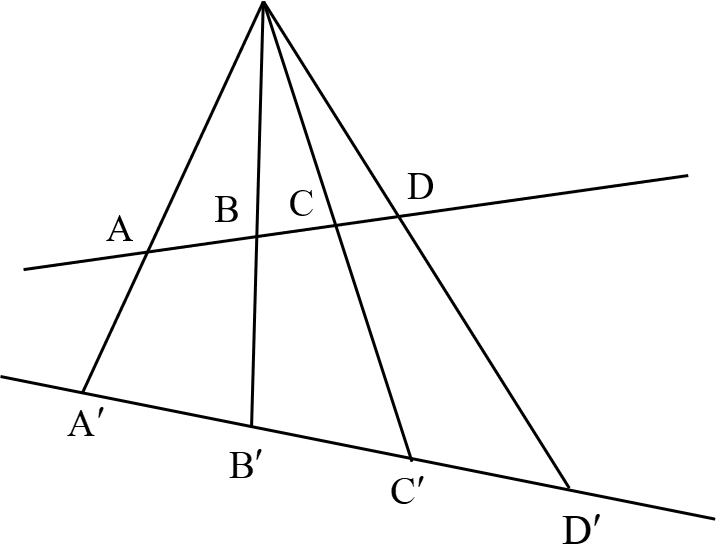
\includegraphics[width=0.5\linewidth]{证明题1.png}
  \caption{射影变换交比不变证明}
\end{figure}\par
交比定义为距离比的比值,在一维空间中的齐次坐标系下,可以使用行列式表示:
$$
  \mathrm{Cross}(A,B,C,D)=\frac{
    \sep AC\sep \sep AD\sep
  }{\sep BC\sep \sep BD\sep }
$$\par
式中,
$$
  \sep AC\sep =\det\begin{bmatrix}
    x_A & x_C \\
    y_A & y_C \\
  \end{bmatrix}
$$\par
是前两项的行列式,因此可设:
$$
  \begin{aligned}
    \mathbold{A}'=s_1\mathbold{HA} \\
    \mathbold{B}'=s_2\mathbold{HB} \\
    \mathbold{C}'=s_3\mathbold{HC} \\
    \mathbold{D}'=s_4\mathbold{HD}
  \end{aligned}
$$\par
代入行列式中,得:
$$
  \begin{aligned}
    \sep A'B'\sep =\det\begin{bmatrix}
                         s_1\mathbold{HA} & s_2\mathbold{HB}
                       \end{bmatrix}=s_1s_2\det(\mathbold{H})\sep AB\sep
  \end{aligned}
$$\par
同理可得:
$$
  \begin{aligned}
    \sep A'C'\sep =s_1s_3\det(\mathbold{H})\sep AC\sep \\
    \sep A'D'\sep =s_1s_4\det(\mathbold{H})\sep AD\sep \\
    \sep B'C'\sep =s_2s_3\det(\mathbold{H})\sep BC\sep \\
    \sep B'D'\sep =s_2s_4\det(\mathbold{H})\sep BD\sep \\
  \end{aligned}
$$\par
代入交比定义,即可验证四个比例因子和行列式$\det\mathbold{H}$均被消去,原式得证。
\subsection{证明仿射变换能把圆映射成椭圆但是不能映射成双曲线和抛物线}
根据二次曲线的仿射分类可知,与无穷远直线没有交点的二次曲线是椭圆或者圆,有一个交点的二次曲线是抛物线,有两个交点的二次曲线是双曲线。仿射变换不改变无穷远直线,而交点性质是射影变换都不会改变的,因此经过仿射变换后,曲线与无穷远直线的交点数量不会变化,所以圆不会变成双曲线和抛物线,而可能变成椭圆。
\subsection{证明仿射变换下平行的两条线段长度之比不变,而不平行的则不然}
设平行线段$AB$和$CD$,则有:
$$
  \begin{aligned}
    \mathbold{A-B}=                    & \lambda(\mathbold{C-D}) \\
    \frac{\sep AB\sep }{\sep CD\sep }= & \lambda
    \label{eq:证明题3}
  \end{aligned}
$$\par
其中$\lambda$为常数,设仿射变换为$\mathbold{X}'=\mathbold{HX}$,则有:
$$
  \mathbold{H}=\begin{bmatrix}
    \mathbold{A} & \mathbold{v} \\
    0            & 1            \\
  \end{bmatrix}
$$\par
当平行线段的端点ABCD不含有无穷远点时,经过仿射变换后,有:
$$
  \begin{aligned}
    \mathbold{A}'=\begin{bmatrix}
                    \mathbold{AX}_A+\mathbold{v}z_A \\
                    z_A
                  \end{bmatrix}
  \end{aligned}
$$\par
因此两平行线段的长度相应地变化为:
$$
  \begin{aligned}
    \sep A'B'\sep = & \sqrt{(\mathbold{X}_A-\mathbold{X}_B)^T\mathbold{A}^T\mathbold{A}(\mathbold{X}_A-\mathbold{X}_B)}        \\
    \sep C'D'\sep = & \sqrt{(\mathbold{X}_C-\mathbold{X}_D)^T\mathbold{A}^T\mathbold{A}(\mathbold{X}_C-\mathbold{X}_D)}        \\
    =               & \lambda\sqrt{(\mathbold{X}_A-\mathbold{X}_B)^T\mathbold{A}^T\mathbold{A}(\mathbold{X}_A-\mathbold{X}_B)} \\
  \end{aligned}
$$\par
因此两线段长度之比不变。对于不平行的线段,由于公式\ref{eq:证明题3}不成立,因此其长度之比不能保持不变。
\subsection{	在二维射影变换中,证明存在一个变换使得单位圆作为集合不变。}
在二维射影变换作用下,单位圆的变换为:
\begin{equation*}
  s\mathbold{C}=\mathbf{H}^{-T}\mathbf{CH}^{-1}
\end{equation*}\par
其中的$\mathbf{C}$满足:
\begin{equation*}
  \mathbf{C}=\begin{bmatrix}
    1 & 0 & 0  \\
    0 & 1 & 0  \\
    0 & 0 & -1
  \end{bmatrix}
\end{equation*}\par
因此可取$\mathbf{H}$为$\mathbf{C}$的相似变换矩阵,而矩阵$\mathbf{C}$是实对称矩阵,它是可以相似对角化的,因此这样的射影变换矩阵是一定存在的。
\subsection{给出极点在椭圆内部的绘图方法}
\begin{figure}[H]
  \centering
  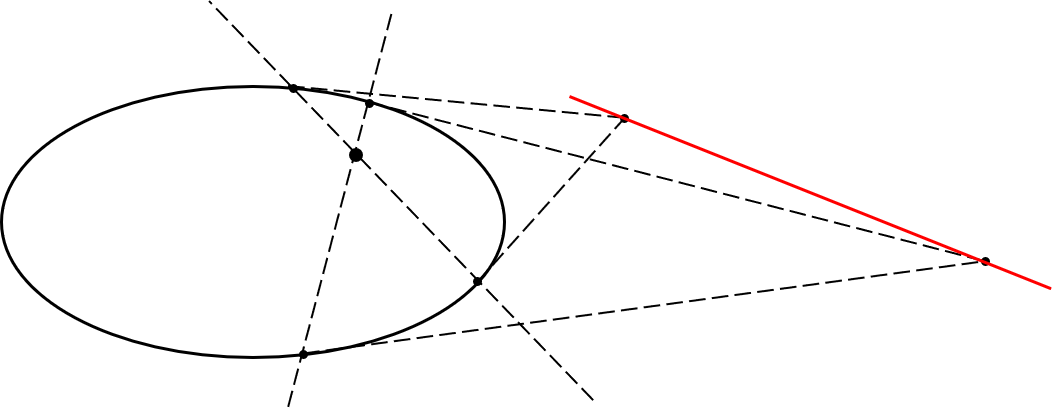
\includegraphics[width=0.5\linewidth]{证明题4.png}
  \caption{射影变换交比不变证明}
  \label{fig:证明题4}
\end{figure}\par
如图\ref{fig:证明题4}所示,过椭圆内部一点任意作两割线,交椭圆于四点,过两割线的对应两点作切线交于两点,连接两点得直线即是椭圆内该点的共轭极线。说明:椭圆的极点极线具有共轭关系,因此过椭圆内一点作的直线与椭圆外一点存在共轭关系,一条直线并不能确定椭圆内的一点,因此需要作两条直线即可确定该极点,而极线上任意一点的极线都经过椭圆内的同一点,这就说明该点就是与极线共轭的极点。
\subsection{证明无穷远平面是绝对对偶二次曲面的零化向量。}
在标准情况下,无穷远平面的方程为:
\begin{equation*}
  \mathbold{\pi}_\infty=\begin{bmatrix}
    0 \\0\\0\\1
  \end{bmatrix}
\end{equation*}\par
绝对对偶二次曲面的方程为:
\begin{equation*}
  \mathbold{Q}^*_\infty=\begin{bmatrix}
    1 & 0 & 0 & 0 \\
    0 & 1 & 0 & 0 \\
    0 & 0 & 1 & 0 \\
    0 & 0 & 0 & 0
  \end{bmatrix}
\end{equation*}\par
显然二者满足:
\begin{equation*}
  \mathbold{Q}^*_\infty\mathbold{\pi}_\infty=0
\end{equation*}\par
在施加射影变换的作用下,绝对对偶二次曲面将变化为:
\begin{equation*}
  {\mathbf{Q'}^*_\infty}=\mathbold{H}\mathbold{Q}^*_\infty\mathbold{H}^T
\end{equation*}\par
而无穷远平面将变化为:
\begin{equation*}
  \mathbold{\pi}_\infty'=\mathbold{H}^{-T}\mathbold{\pi}_\infty
\end{equation*}\par
因此有:
\begin{equation*}
  {\mathbold{Q}^*_\infty}'{\mathbold{\pi}_\infty}'=\mathbold{H}\mathbold{Q}^*_\infty\mathbold{H}^T\mathbold{H}^{-T}\mathbold{\pi}_\infty=\mathbold{H}\mathbold{Q}^*_\infty\mathbold{\pi}_\infty=\mathbold{0}
\end{equation*}\par
因此在任意情况下,无穷远平面均是绝对对偶二次曲面的零化向量。
\subsection{利用Plücker直线坐标写出关于直线与平面交点的表示式以及由一点与一直线定义的平面的表示式}
直线与平面$\mathbold{\pi}$的交点可写为:
\begin{equation*}
  \mathbold{X}=\mathbold{L}\mathbold{\pi}
\end{equation*}\par
证明该点同时位于直线上和平面上:
设直线的plücker表达式为:
\begin{equation*}
  \mathbold{L}=\mathbf{AB}^T-\mathbf{BA}^T\qquad\mathbf{L}^*=\mathbf{PQ}^T-\mathbf{QP}^T
\end{equation*}\par
其中$\mathbf{A,B}$为直线上的两点,位于平面$\mathbf{P,Q}$上,则有:
\begin{equation*}
  \mathbf{P}^T\mathbf{A}=\mathbf{P}^T\mathbf{B}=\mathbf{Q}^T\mathbf{A}=\mathbf{Q}^T\mathbf{B}=0
\end{equation*}\par
因此有:
\begin{align*}
  \mathbf{L^*X} & =\circbrac{\mathbf{PQ}^T-\mathbf{QP}^T}\circbrac{\mathbf{AB}^T-\mathbf{BA}^T}\mathbf{X}                                                              \\
                & =\mathbf{PQ}^T\mathbf{AB}^T\mathbf{X}-\mathbf{PQ}^T\mathbf{BA}^T\mathbf{X}-\mathbf{QP}^T\mathbf{AB}^T\mathbf{X}+\mathbf{QP}^T\mathbf{BA}^T\mathbf{X} \\
                & =\mathbf{0}
\end{align*}\par
可见该点位于直线上,同理:
\begin{align*}
  \mathbold{\pi}^T\mathbf{X}= & \mathbold{\pi}^T\mathbf{L}\mathbold{\pi}                                               \\
                              & =\mathbold{\pi}^T\circbrac{\mathbf{AB}^T-\mathbf{BA}^T}\mathbold{\pi}                  \\
                              & =\mathbold{A^\mathrm{T}\pi B^\mathrm{T}\pi}-\mathbold{B^\mathrm{T}\pi A^\mathrm{T}\pi} \\
                              & =\mathbf{0}
\end{align*}\par
式中用到了内积为纯量因此可以交换位置的性质,而交换后恰好让两式归0,因此该点同时位于直线和平面上。\par
同理,由一点与一条直线定义的平面表达式为:
\begin{equation*}
  \mathbold{\pi}=\mathbold{L^*}\mathbold{X}
\end{equation*}\par
证明方法类似,不再赘述。
\subsection{利用plucker坐标推导点在直线上和直线在平面上的条件}
点在直线上的条件:
\begin{equation*}
  \mathbf{L^*X}=\mathbf{0}
\end{equation*}\par
证明方法是说明该点即在平面$\mathbf{P}$又在平面$\mathbf{Q}$上说明的;\par
直线在平面上的条件:
\begin{equation*}
  \mathbold{L\pi}=\mathbf{0}
\end{equation*}\par
证明方法是通过直线上某两点在平面上说明的。
\subsection{利用Plücker坐标证明平行平面相交在无穷远平面上的一条直线上}
设两平行平面为:
\begin{align*}
  \mathbold{\pi}_1=\begin{bmatrix}
                     a \\b\\c\\d_1
                   \end{bmatrix}\qquad\mathbold{\pi}_2=\begin{bmatrix}
                                                         a \\b\\c\\d_2
                                                       \end{bmatrix}
\end{align*}\par
然后计算出来即可说明用该两平面生成的直线位于无穷远平面上。
\subsection{证明平行线相交在无穷远平面上}
证明思路:参考自\cite{MultipleViewGeometrya},两平行直线必定是共面的,因此可构造两个平行平面依次与公共平面相交于两平行直线处,根据上文证明,两平行平面交于无穷远平面,而公共平面与无穷远平面有交线,因此两平行直线与无穷远平面的交点必定是公共平面交线和平行平面交线的交集,因此该点位于无穷远平面上。
\subsection{证明绝对对偶二次曲面是绝对二次曲线的对偶(对偶即二次曲线的切面被二次曲面的包络)}
在标准情况下绝对二次曲线和绝对对偶二次曲面都是如下的矩阵:
\begin{equation*}
  \mathbold{\Omega}_\infty=\mathbold{Q}^*_\infty=\begin{bmatrix}
    1 & 0 & 0 & 0 \\
    0 & 1 & 0 & 0 \\
    0 & 0 & 1 & 0 \\
    0 & 0 & 0 & 0
  \end{bmatrix}
\end{equation*}\par
在标准情况下,绝对二次曲线的切线方程为:
\begin{equation*}
  \mathbold{l}=\mathbold{\Omega}_\infty\mathbold{X}=\begin{bmatrix}
    \mathbf{I}   & 0 \\
    \mathbf{0}^T & 0
  \end{bmatrix}\begin{bmatrix}
    \mathbf{v} \\ 0
  \end{bmatrix}=\begin{bmatrix}
    \mathbf{v} \\ 0
  \end{bmatrix}
\end{equation*}\par
由于切点在绝对二次曲线上,因此满足:
\begin{equation*}
  \mathbold{v}^T\mathbold{v}=0
\end{equation*}\par
因此,切线满足以下方程:
\begin{equation*}
  \mathbf{l}^T\mathbf{Q}_\infty^*\mathbf{l}=\mathbf{v}^T\mathbf{v}=0
\end{equation*}\par
说明绝对对偶二次曲线是绝对二次曲线的对偶。当外加射影变换矩阵作用后,无穷远平面产生协变,因此绝对二次曲线产生协变,绝对对偶二次曲面产生变换,分别为:
\begin{equation*}
  \mathbold{\Omega}_\infty'=\mathbold{H}^{-T}\mathbold{\Omega}_\infty\mathbold{H}^{-1}\qquad\mathbf{Q'}_\infty^{*}=\mathbold{H}\mathbold{Q}_\infty^*\mathbold{H}^T
\end{equation*}\par
因此,绝对二次曲线的切线方程变为:
\begin{equation*}
  \mathbold{l}'=\mathbf{H}^{-T}\mathbf{l}
\end{equation*}\par
其符合变换后的绝对对偶二次曲面方程:
\begin{equation*}
  \mathbf{l'}^T\mathbf{Q'}_\infty^{*}\mathbf{l'}=\mathbf{l}^T\mathbf{H}^{-1}\mathbf{H}\mathbf{Q}_\infty^*\mathbf{H}^T\mathbf{H}^{-T}\mathbf{l}=\mathbf{l}^T\mathbf{Q}_\infty^*\mathbf{l}=0
\end{equation*}\par
因此在任意情况下,绝对对偶二次曲面都是绝对二次曲线的对偶。
\subsection{证明绝对对偶二次曲面不变射影变换是相似变换,反之也成立}
证明思路:用标准情况下的绝对对偶二次曲面(秩亏单位阵)和一般情况下的的射影变换阵,然后证明变换后的绝对对偶二次曲面阵与原始阵相同,因此可推出射影变换阵的$\mathbf{A}$子块是正交矩阵,同时也可以得出$\mathbf{v}^T\mathbf{v}=0$,推出矢量$\mathbf{v}$是零向量,因此射影变换矩阵是相似变换阵。
\subsection{证明过点x的二次曲线切线是Cx}
这是二维齐次坐标下的证明,可反设过$\mathbf{x}$点直线还交二次曲线于$\mathbf{y}$点,即有:
\begin{equation*}
  \mathbf{x}^T\mathbf{Qx}=\mathbf{y}^T\mathbf{Qy}=0
\end{equation*}\par
因此可通过线性叠加证明经过$\mathbf{x,y}$的全部点的直线都在二次曲线上,与二次曲线不退化的前提矛盾,因此$\mathbf{y}$点不可能存在,即$\mathbf{x}$点的切线是$\mathbf{Cx}$。
\subsection{证明过点X的二次曲面切平面是QX}
与上一问的证明方式一模一样,不再赘述。
\subsection{蒙娜丽莎的眼睛}
{\heiti 设是$I_0$射影图像,而$I_1$是$I_0$的图像,其合成图像为$I'$,证明$I'$的视在摄像机中心与$I_0$的一样,并验证$I'$和$I_0$的其他参数可能不同。}\par
这个题题意不明,查阅资料\cite{MultipleViewGeometry}后才知道,合成图像应该就是$I_0$的意思,只不过$I_1$和$I_0$是针对不同摄像机而言的。一般的射影摄像机模型为:
\begin{equation*}
  \mathbold{P}=\mathbold{KR[I\sep -\tilde{C}]}
\end{equation*}\par
对原始射影场景$I_0$生成得到的图像$I_1$为:
\begin{equation*}
  \mathbold{x}_0=\mathbold{KRP}^{-1}\mathbold{X}_\mathrm{cam}
\end{equation*}\par
而人眼相当于一套双目摄像机,其对图像$I_1$成像,相当于一个二维的单应变换,将该单应叠加至投影成像中,可得:
\begin{equation*}
  \mathbold{x}_1=\mathbold{HKR[I\sep -\tilde{C}]}\mathbold{X}_\mathrm{cam}
\end{equation*}\par
可见,合成图像中的摄像机中心仍然与原始摄像机中心一致,在世界坐标系下均为$\tilde{\mathbf{C}}$,而其他参数如摄像机矩阵等均受到二次投影的影响,因此可能不同。\par
因此,蒙娜丽莎的眼睛始终看着观察者,原因在于,观察者的眼睛相当于一个射影摄像机,蒙娜丽莎图像本身可以相当于一幅射影摄像机的图像,画中蒙娜丽莎的眼睛始终看着摄像机的中心,而观察者对该图像的二次成像不改变摄像机中心,所以看起来蒙娜丽莎在观察者眼中成像后的图像中的眼睛始终看着观察者。
\subsection{射影摄像机反向投影}
{\heiti 证明在射影摄像机下,图像点的反向投影的射线可以被写成$\mathbf{L}^*=\mathbf{P}^T\mathbf{[x]_\times P}$}\par
过图像点$\mathbf{x}$,在图像上任作两直线$\mathbf{l}_1,\mathbf{l}_2$,利用射影摄像机对直线的反向投影,可得:
\begin{align*}
  \mathbold{\pi}_1=\mathbf{P}^T\mathbf{l}_1 & \qquad\mathbold{\pi}_2=\mathbf{P}^T\mathbf{l}_2                                   \\
  \mathbf{x}=\mathbf{l}_1\times\mathbf{l}_2 & \implies\mathbf{[x]_\times}=\mathbf{l}_1\mathbf{l}_2^T-\mathbf{l}_1\mathbf{l}_2^T
\end{align*}\par
因此,利用Plücker坐标的定义,可得:
\begin{equation*}
  \mathbf{L}^*=\mathbold{\pi}_1\mathbold{\pi}_2^T-\mathbold{\pi}_2\mathbold{\pi}_1^T=\mathbf{P}^T\mathbf{l}_1\mathbf{l}_2^T\mathbf{P}-\mathbf{P}^T\mathbf{l}_2\mathbf{l}_1^T\mathbf{P}=\mathbf{P}^T\mathbf{[x]_\times P}
\end{equation*}\par
\subsection{证明仿射摄像机是可以将平行的世界直线映射为平行的图像直线的关于齐次坐标的最一般的线性映射}
证明思路:任取无穷远平面上的一点$\mathbf{X}_\infty$,对其作投影变换,其在图像平面上的应该也位于无穷远直线上,可得:
\begin{equation*}
  \mathbf{x}_\infty=\begin{bmatrix}
    x \\y\\0
  \end{bmatrix}=\mathbf{P}\mathbf{X}_\infty
\end{equation*}\par
因此可知:
\begin{equation*}
  p_{31}X+p_{32}Y+p_{33}Z+p_{34}\times0=0
\end{equation*}\par
现根据该无穷远点的任意性,上式恒成立,因此可得:
\begin{equation*}
  p_{31}=p_{32}=p_{33}=0,p_{34}\neq0
\end{equation*}\par
因此证明投影矩阵具有以下形式:
\begin{equation*}
  \mathbf{P}=\begin{bmatrix}
    p_{11} & p_{12} & p_{13} & p_{14} \\
    p_{21} & p_{22} & p_{23} & p_{24} \\
    0      & 0      & 0      & p_{34}
  \end{bmatrix}
\end{equation*}\par
说明该摄像机是仿射摄像机。
\subsection{重要公式之一}
{\heiti 经相机矩阵$\mathbf{P}$映射成一条直线$\mathbf{l}$的空间点集是平面$\mathbf{P}^T\mathbf{l}$}。\par
\textbr{超级简单,但是超级经典!}\par
在空间中任取一点$\mathbf{X}$,其射影点$\mathbf{x=PX}$落在直线$\mathbf{l}$上,因此有:
\begin{equation*}
  \mathbf{l}^T\mathbf{x}=\mathbf{l}^T\mathbf{PX}=0
\end{equation*}\par
可取后式的前半项为对应的平面,因此证得:
\begin{equation*}
  \mathbf{P}^T\mathbf{l}=\mathbold{\pi}
\end{equation*}\par
为所求的反投影平面。
\subsection{重要公式之二}
{\heiti 图像直线$\mathbf{l}$能够确定一张过摄像机中心的平面,该平面的法线方向为$\mathbf{n=K^\mathit{T}l}$}。\par
\textbr{超级简单,但是注意引论!}\par
证明该结论首先应当证明一个引论,即射影摄像机将图像平面上的点反向投影为直线的方向向量为:
\begin{equation*}
  \mathbf{x}=\mathbf{K[I\sep 0]}\begin{bmatrix}
    \lambda\mathbf{d} \\1
  \end{bmatrix}
\end{equation*}\par
因此可知该方向向量为:
\begin{equation*}
  \mathbf{d}=\mathbf{K}^{-1}\mathbf{x}
\end{equation*}\par
因此,图像点在图像直线上,有:
\begin{equation*}
  \mathbf{l^\mathit{T}x}=\mathbf{l^\mathit{T}K}\mathbf{d}=0
\end{equation*}\par
此式解出了与直线的方向向量正交的向量,该向量就是平面的法向量,因此可得:
\begin{equation*}
  \mathbf{n}=\mathbf{K}^T\mathbf{l}
\end{equation*}\par
\subsection{平面全景拼图的步骤,为什么会产生黑边(原文:蝴蝶结形状)}
书上原话:因为所有的图像都是往中间一幅图像配准所得的,因此两侧的图像射影变换产生的拉伸较大,而靠近中间的射影变换拉伸较小,因此两头大中间小,产生了黑边(或蝴蝶结的形状)。
\subsection{空间绝对二次曲线的图像}
{\heiti 证明空间中绝对二次曲线的图像是$\circbrac{\mathbf{KK}^{T}}^{-1}$}\par
空间的绝对二次曲线位于无穷远平面上,因此考虑使用无穷远平面向图像平面的二维单应解决此问题。设无穷远平面上的一点为$\mathbf{X}_\infty$,其在图像平面上的投影为${\mathbf{x}_\infty}'$,则有:
\begin{equation*}
  {\mathbf{x}_\infty}'=\mathbf{KR[I\sep} -\tilde{\mathbf{C}}]\begin{bmatrix}
    \mathbf{x}_\infty \\0
  \end{bmatrix}=\mathbf{KRx}_\infty
\end{equation*}\par
所以该二维单应是$\mathbf{H=KR}$,根据二维单应情况下的绝对二次曲线协变,可得图像平面上的绝对二次曲线为:
\begin{equation*}
  \mathbf{C}'=\mathbf{H}^{-T}\mathbf{CH}^{-1}=\mathbf{K^\mathit{-T}R^\mathit{-T}IR^{-1}K^{-1}}=\mathbf{K^\mathit{-T}K^{-1}}
\end{equation*}\par
因为旋转矩阵是正交矩阵,因此可以得到上述结果,由此完成证明。
\subsection{证明使用三条共面的等距平行线可确定图像的消影线}
\textbr{重要前提:}$\mathbf{l_\infty}=a\mathbf{l}_1+b\mathbf{l}_2$\par
在这个重要前提下,可以待定系数$a,b$解出无穷远直线。首先等距直线在原始图像上满足:
\begin{align*}
  \mathbf{l}_1'=\mathbf{l}_0'+\mathbf{l'}_\infty \\
  \mathbf{l}_2'=\mathbf{l}_0'+2\mathbf{l'}_\infty
\end{align*}\par
因此,去除右上标的标记即可得到在失真图像平面上的关系式,即:
\begin{align*}
  \mathbf{l}_1=\mathbf{l}_0+{\mathbf{l}_\infty  } \\
  \mathbf{l}_2=\mathbf{l}_0+{2\mathbf{l}_\infty  }
\end{align*}\par
叉乘重要前提公式有:
\begin{align*}
  \mathbf{l}_\infty\times\mathbf{l}_1 & =b\mathbf{l}_2\times\mathbf{l}_1 \\
  \mathbf{l}_\infty\times\mathbf{l}_2 & =a\mathbf{l}_1\times\mathbf{l}_2
\end{align*}
由此使用内积将矢量转为纯量,可以反解出:
\begin{align*}
  b & =-\frac{\circbrac{\mathbf{l}_2\times\mathbf{l}_1}^T\circbrac{\mathbf{l}_0\times\mathbf{l}_1}}{\circbrac{\mathbf{l}_2\times\mathbf{l}_1}^T\circbrac{\mathbf{l}_2\times\mathbf{l}_1}}            \\
  a & =-\frac{1}{2}\frac{\circbrac{\mathbf{l}_1\times\mathbf{l}_2}^T\circbrac{\mathbf{l}_0\times\mathbf{l}_2}}{\circbrac{\mathbf{l}_1\times\mathbf{l}_2}^T\circbrac{\mathbf{l}_1\times\mathbf{l}_2}}
\end{align*}\par
因此,可以得到无穷远直线的表达式为:
\begin{equation*}
  \mathbf{l}_\infty=-\frac{1}{2}\frac{\circbrac{\mathbf{l}_1\times\mathbf{l}_2}^T\circbrac{\mathbf{l}_0\times\mathbf{l}_2}}{\circbrac{\mathbf{l}_1\times\mathbf{l}_2}^T\circbrac{\mathbf{l}_1\times\mathbf{l}_2}}\mathbf{l}_1-\frac{\circbrac{\mathbf{l}_2\times\mathbf{l}_1}^T\circbrac{\mathbf{l}_0\times\mathbf{l}_1}}{\circbrac{\mathbf{l}_2\times\mathbf{l}_1}^T\circbrac{\mathbf{l}_2\times\mathbf{l}_1}}\mathbf{l}_2
\end{equation*}\par
叉乘满足反交换律,因此约去齐次的比例因子可得:
\begin{equation*}
  \mathbf{l}_\infty=\circbrac{\mathbf{l}_1\times\mathbf{l}_2}^T\circbrac{\mathbf{l}_0\times\mathbf{l}_2}\mathbf{l}_1+2\circbrac{\mathbf{l}_2\times\mathbf{l}_1}^T\circbrac{\mathbf{l}_0\times\mathbf{l}_1}\mathbf{l}_2
\end{equation*}\par
即为所求。
\subsection{证明空间直线的正投影公式}
{\heiti 证明空间直线的正投影公式为$\mathbf{[l]}_\times=\mathbf{P}\mathbf{LP}^T$}\par
在空间直线上任取两点,使用投影变换算出其在图像平面上的投影点,然后利用投影点的扩展叉乘公式即可证明该公式。
\subsection{证明通过摄像机中心的空间直线被投影为零向量}
在空间直线上任取一点$\mathbf{X}$,表示该直线为:
\begin{equation*}
  \mathbf{L}=\mathbf{CX}^{T}-\mathbf{XC}^T
\end{equation*}\par
代入上述正投影公式,可得:
\begin{equation*}
  \mathbf{[l]}_\times=\mathbf{0}
\end{equation*}
因此该图像直线是零向量。
\subsection{火车为什么远处运动慢而近处运动快?}
\label{subsec:火车为什么远处运动慢而近处运动快?}
\textbr{提醒:本题需要用到二视图}\par
设空间中一点的非齐次坐标为:$\mathbf{X}=[X,Y,Z]^T$,人眼相当于一个摄像机,投影矩阵的模型为$\mathbf{P=K[I\sep 0]}$,因此成像在视网膜上的图像齐次坐标为:
\begin{equation*}
  \mathbf{x}=\mathbf{K[I\sep 0]}\begin{bmatrix}
    X \\Y\\Z\\1
  \end{bmatrix}\implies \mathbf{K}\begin{bmatrix}
    X \\Y\\Z
  \end{bmatrix}=s\begin{bmatrix}
    x \\y\\1
  \end{bmatrix}
\end{equation*}\par
式中的$s$是齐次因子,如果取定人眼的内参数矩阵$K_{33}=1$,则该齐次因子可定为$s={Z}$。当人沿着X轴方向行进一小段距离后,则人眼摄像机在同一个世界坐标系下产生的平移向量为$\mathbf{t}=\begin{bmatrix}
    \Delta X \\0\\0
  \end{bmatrix}$,则有:
在新的相机投影矩阵下,该点的投影为:
\begin{equation*}
  \mathbf{x}'=\mathbf{K[I\sep t]}\begin{bmatrix}
    X \\Y\\Z\\1
  \end{bmatrix}\implies \mathbf{K}\begin{bmatrix}
    X \\Y\\Z
  \end{bmatrix}=s'\begin{bmatrix}
    x' \\y'\\1
  \end{bmatrix}
\end{equation*}\par
由于内参数矩阵是上三角阵,因此原式等于:
\begin{equation*}
  s'\begin{bmatrix}
    x' \\y'\\1
  \end{bmatrix}=\mathbf{K}\begin{bmatrix}
    X+\Delta X \\Y\\Z
  \end{bmatrix}
\end{equation*}
根据右式右下角元素为$Z$,可计算出$s'=Z$,因此将上式改写为:
\begin{equation*}
  \begin{bmatrix}
    x' \\y'\\1
  \end{bmatrix}=\begin{bmatrix}
    x \\y\\1
  \end{bmatrix}+\frac{1}{Z}\begin{bmatrix}
    \Delta X \\0\\0
  \end{bmatrix}
\end{equation*}\par
可见,在X轴方向的运动上,当深度越大时,视在的运动量越小,因此坐火车时,火车运动方向相当于是X轴运动,距离车窗较远的场景点深度较大,其视在运动越慢,而距离车窗较近的场景点深度较小,其视在运动越快。
\subsection{证明虚圆点相对相似变换不变}
二维的结论是显然的,对于三维:三维的映射不是点点不变的,而是集合不变,因此证明该结论只能通过标准情况+射影变换证得。
\section{练习题答案}
\subsection{使用一条消影直线和一个消影点对应和基本矩阵可算出仿射重构}
\textbr{说明:}这里的一条消影直线对应和一个消影点对应分别指的是左右相机各有一条消影直线和同一个消影点的像,消影点不在消影线上(空间无穷远平面不过摄像机中心)。\par
思路:$\mathbf{H}_\infty$共有8个独立的参数,因此需要想办法取得4对不同的对应点。这里,在左图的消影线上任取两点,使用对极线约束$\mathbf{l}_r=\mathbf{Fx}_l$可以算出右图的两条对极线,又因为两个点均在消影线上,因此右图中的两条对极线分别与消影线向量积可以求出右图中对应 的两个消影点,由此得到了两个对应点约束。(此时不能从消影线上再取点得到对应点了,因为再取的点将与这两个点线性相关,约束是无效的)。\par
然后可通过基本矩阵的左零空间和右零空间,算出两个对极点:
\begin{equation*}
  \mathbf{Fe}_l=0\qquad\mathbf{e}_r^T\mathbf{F}=0
\end{equation*}\par
加上题目中给出的不共线消影点约束,即可得到四个对应点约束,方程:
\begin{equation*}
  \mathbf{x}_r=\mathbf{H}_\infty \mathbf{x}_l
\end{equation*}\par
在齐次意义下存在唯一解。
\subsection{坐在一个旋转木马上旋转,观察到的远处的景物和近处的景物有什么差别?}
\textbr{提醒:对结论\ref{subsec:火车为什么远处运动慢而近处运动快?}的扩展,牢记双目推导法。}\par
设旋转木马上旋转前后的人眼摄像机的投影矩阵分别为$\mathbf{P}_1,\mathbf{P}_2$,则有:
\begin{equation*}
  \mathbf{P}_1=\mathbf{K[I\sep 0]}\qquad\mathbf{P}_2=\mathbf{K[R\sep t ]} 
\end{equation*}\par
图像点为$\mathbf{x}=[x,y,1]^T$,则在世界坐标系下的世界点为:
\begin{equation*}
  \mathbf{X}=\begin{bmatrix}
    X \\Y\\Z\\1
  \end{bmatrix}=Z\mathbf{K^\mathrm{-1}x}
\end{equation*}\par
则在旋转后的成像为:
\begin{align*}
  Z\mathbf{x}'=\mathbf{P}_2\mathbf{X}=\mathbf{K[R\sep t ]}\mathbf{X}&=Z\mathbf{KRK^\mathrm{-1}x}+Z\mathbf{Kt}\\
  \mathbf{x}'=\mathbf{KRK^\mathrm{-1}x}+\frac{\mathbf{K^\mathrm{-1}t}}{Z}
\end{align*}\par
因此世界点的视在旋转量相同,但是视在平移量与深度呈反比,距离人越远的点,给人的感觉是运动越慢,越近的人运动越快。
\subsection{提出一种利用标定二次曲线标定摄像机的方法}
\textbr{提醒:}这里的标定二次曲线是指世界坐标已知的二次曲线。\par
该方法较为复杂,标定板上必须有至少两个圆,圆的半径可以不相等,标定思路是首先利用两个圆求解出无穷远直线,然后通过两组垂直线解出仿射矩阵,对拼合起来的矩阵使用QR分解,上三角阵就是待标定的摄像机矩阵。\par
在摄像机的作用下,标定板到图像存在一个二维单应,即:
\begin{equation}
  \mathbf{H=KR}=\begin{bmatrix}
    \mathbf{I}&\mathbf{0}\\
    \mathbf{v}^T&v_3
  \end{bmatrix}\begin{bmatrix}
    \mathbf{K}&\mathbf{0}\\
    \mathbf{0}^T&1
  \end{bmatrix}\begin{bmatrix}
    s\mathbf{R}&\mathbf{t}\\
    \mathbf{0}^T&1
  \end{bmatrix}
  \label{eq:标定板到图像的二维单应}
\end{equation}\par
\begin{figure}[H]
  \centering
  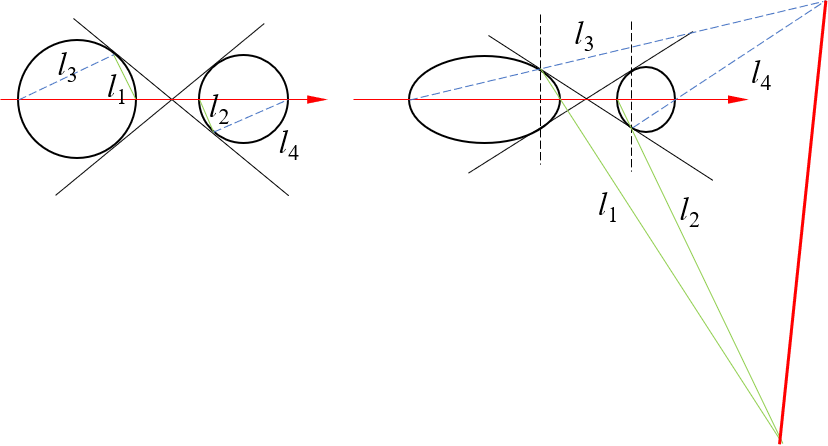
\includegraphics[width=0.8\linewidth]{练习题5.png}
  \caption{两个标定圆求解无穷远直线}
\label{fig:两个标定圆求解无穷远直线}
\end{figure}\par
如图\ref{fig:两个标定圆求解无穷远直线},在图像平面上,作两个圆长轴的连线,作内公切线得到四个切线,连接对应的切点,可得两条平行线。这两条平行线在世界坐标系下应该是相交的,因此可以求出无穷远直线,使用该无穷远直线和任意一个圆的影像求出虚圆点,使用虚圆点还原绝对二次曲线,从而获取绝对对偶二次曲线,使用奇异值分解可算出单应矩阵$\mathbf{H}$,对单应矩阵作QR分解可得标定矩阵$\mathbf{K}$。(本方法将求解非线性方程)\par
为了避免求解非线性方程,可选取两对正交直线,使用仿射校正矩阵$\begin{bmatrix}
  \mathbf{I}&\mathbf{0}\\
  \mathbf{v}^T&v_3
\end{bmatrix}$
将直线校正后,通过下式解出矩阵$\mathbf{K}$:
\begin{equation*}
  \rectbrac{l_1,l_2,l_3}\begin{bmatrix}
    \mathbf{KK}^T&\mathbf{0}\\
    \mathbf{0}^T&1
  \end{bmatrix}\begin{bmatrix}
    m_1\\
    m_2\\
    m_3
  \end{bmatrix}
\end{equation*}\par
然后作Cholesky分解可求得矩阵$K$,从而利用公式\ref{eq:标定板到图像的二维单应}可在相差一个相似变换的情况下求得$\mathbf{H}$,该结果对QR分解不影响,因此完成标定。
\subsection{给出一种用消隐线求解摄像机旋转的方法}
以旋转前的相机为世界坐标系,旋转后所得的图像可由单应矩阵$\mathbf{H}$联系,即:
\begin{equation*}
  \mathbf{H}=\mathbf{KRK}^{-1}
\end{equation*}\par
其中旋转矩阵共有三个自由度,因此至少需要两组对应的消隐点即可完成旋转求解。这里必须先验摄像机的内参数矩阵$\mathbf{K}$,相机图像中的绝对二次曲线的图像为:
\begin{equation*}
  \mathbold{\omega}=\mathbf{K}^{-T}\mathbf{K}^{-1}
\end{equation*}\par
在旋转前图像的消隐线上选择一点$\mathbf{x}$,其满足旋转的极点极线约束并在旋转后图像的消隐线上,有:
\begin{equation*}
  \mathbf{l}'=\mathbold{\omega x}\qquad\mathbf{l}'\times\mathbf{l'}_\infty=\mathbf{x'}
\end{equation*}\par
由此可以两组对应点,能够解出旋转矩阵。
\subsection{一个矩形的标定物体平行移动为什么不能实现摄像机的标定?}
\newpage
\printbibliography[heading=bibliography,title=参考文献]
\end{document}